% Options for packages loaded elsewhere
\PassOptionsToPackage{unicode}{hyperref}
\PassOptionsToPackage{hyphens}{url}
\PassOptionsToPackage{dvipsnames,svgnames,x11names}{xcolor}
%
\documentclass[
  letterpaper,
  DIV=11,
  numbers=noendperiod]{scrartcl}

\usepackage{amsmath,amssymb}
\usepackage{iftex}
\ifPDFTeX
  \usepackage[T1]{fontenc}
  \usepackage[utf8]{inputenc}
  \usepackage{textcomp} % provide euro and other symbols
\else % if luatex or xetex
  \usepackage{unicode-math}
  \defaultfontfeatures{Scale=MatchLowercase}
  \defaultfontfeatures[\rmfamily]{Ligatures=TeX,Scale=1}
\fi
\usepackage{lmodern}
\ifPDFTeX\else  
    % xetex/luatex font selection
\fi
% Use upquote if available, for straight quotes in verbatim environments
\IfFileExists{upquote.sty}{\usepackage{upquote}}{}
\IfFileExists{microtype.sty}{% use microtype if available
  \usepackage[]{microtype}
  \UseMicrotypeSet[protrusion]{basicmath} % disable protrusion for tt fonts
}{}
\makeatletter
\@ifundefined{KOMAClassName}{% if non-KOMA class
  \IfFileExists{parskip.sty}{%
    \usepackage{parskip}
  }{% else
    \setlength{\parindent}{0pt}
    \setlength{\parskip}{6pt plus 2pt minus 1pt}}
}{% if KOMA class
  \KOMAoptions{parskip=half}}
\makeatother
\usepackage{xcolor}
\setlength{\emergencystretch}{3em} % prevent overfull lines
\setcounter{secnumdepth}{-\maxdimen} % remove section numbering
% Make \paragraph and \subparagraph free-standing
\ifx\paragraph\undefined\else
  \let\oldparagraph\paragraph
  \renewcommand{\paragraph}[1]{\oldparagraph{#1}\mbox{}}
\fi
\ifx\subparagraph\undefined\else
  \let\oldsubparagraph\subparagraph
  \renewcommand{\subparagraph}[1]{\oldsubparagraph{#1}\mbox{}}
\fi

\usepackage{color}
\usepackage{fancyvrb}
\newcommand{\VerbBar}{|}
\newcommand{\VERB}{\Verb[commandchars=\\\{\}]}
\DefineVerbatimEnvironment{Highlighting}{Verbatim}{commandchars=\\\{\}}
% Add ',fontsize=\small' for more characters per line
\usepackage{framed}
\definecolor{shadecolor}{RGB}{248,248,248}
\newenvironment{Shaded}{\begin{snugshade}}{\end{snugshade}}
\newcommand{\AlertTok}[1]{\textcolor[rgb]{0.94,0.16,0.16}{#1}}
\newcommand{\AnnotationTok}[1]{\textcolor[rgb]{0.56,0.35,0.01}{\textbf{\textit{#1}}}}
\newcommand{\AttributeTok}[1]{\textcolor[rgb]{0.13,0.29,0.53}{#1}}
\newcommand{\BaseNTok}[1]{\textcolor[rgb]{0.00,0.00,0.81}{#1}}
\newcommand{\BuiltInTok}[1]{#1}
\newcommand{\CharTok}[1]{\textcolor[rgb]{0.31,0.60,0.02}{#1}}
\newcommand{\CommentTok}[1]{\textcolor[rgb]{0.56,0.35,0.01}{\textit{#1}}}
\newcommand{\CommentVarTok}[1]{\textcolor[rgb]{0.56,0.35,0.01}{\textbf{\textit{#1}}}}
\newcommand{\ConstantTok}[1]{\textcolor[rgb]{0.56,0.35,0.01}{#1}}
\newcommand{\ControlFlowTok}[1]{\textcolor[rgb]{0.13,0.29,0.53}{\textbf{#1}}}
\newcommand{\DataTypeTok}[1]{\textcolor[rgb]{0.13,0.29,0.53}{#1}}
\newcommand{\DecValTok}[1]{\textcolor[rgb]{0.00,0.00,0.81}{#1}}
\newcommand{\DocumentationTok}[1]{\textcolor[rgb]{0.56,0.35,0.01}{\textbf{\textit{#1}}}}
\newcommand{\ErrorTok}[1]{\textcolor[rgb]{0.64,0.00,0.00}{\textbf{#1}}}
\newcommand{\ExtensionTok}[1]{#1}
\newcommand{\FloatTok}[1]{\textcolor[rgb]{0.00,0.00,0.81}{#1}}
\newcommand{\FunctionTok}[1]{\textcolor[rgb]{0.13,0.29,0.53}{\textbf{#1}}}
\newcommand{\ImportTok}[1]{#1}
\newcommand{\InformationTok}[1]{\textcolor[rgb]{0.56,0.35,0.01}{\textbf{\textit{#1}}}}
\newcommand{\KeywordTok}[1]{\textcolor[rgb]{0.13,0.29,0.53}{\textbf{#1}}}
\newcommand{\NormalTok}[1]{#1}
\newcommand{\OperatorTok}[1]{\textcolor[rgb]{0.81,0.36,0.00}{\textbf{#1}}}
\newcommand{\OtherTok}[1]{\textcolor[rgb]{0.56,0.35,0.01}{#1}}
\newcommand{\PreprocessorTok}[1]{\textcolor[rgb]{0.56,0.35,0.01}{\textit{#1}}}
\newcommand{\RegionMarkerTok}[1]{#1}
\newcommand{\SpecialCharTok}[1]{\textcolor[rgb]{0.81,0.36,0.00}{\textbf{#1}}}
\newcommand{\SpecialStringTok}[1]{\textcolor[rgb]{0.31,0.60,0.02}{#1}}
\newcommand{\StringTok}[1]{\textcolor[rgb]{0.31,0.60,0.02}{#1}}
\newcommand{\VariableTok}[1]{\textcolor[rgb]{0.00,0.00,0.00}{#1}}
\newcommand{\VerbatimStringTok}[1]{\textcolor[rgb]{0.31,0.60,0.02}{#1}}
\newcommand{\WarningTok}[1]{\textcolor[rgb]{0.56,0.35,0.01}{\textbf{\textit{#1}}}}

\providecommand{\tightlist}{%
  \setlength{\itemsep}{0pt}\setlength{\parskip}{0pt}}\usepackage{longtable,booktabs,array}
\usepackage{calc} % for calculating minipage widths
% Correct order of tables after \paragraph or \subparagraph
\usepackage{etoolbox}
\makeatletter
\patchcmd\longtable{\par}{\if@noskipsec\mbox{}\fi\par}{}{}
\makeatother
% Allow footnotes in longtable head/foot
\IfFileExists{footnotehyper.sty}{\usepackage{footnotehyper}}{\usepackage{footnote}}
\makesavenoteenv{longtable}
\usepackage{graphicx}
\makeatletter
\def\maxwidth{\ifdim\Gin@nat@width>\linewidth\linewidth\else\Gin@nat@width\fi}
\def\maxheight{\ifdim\Gin@nat@height>\textheight\textheight\else\Gin@nat@height\fi}
\makeatother
% Scale images if necessary, so that they will not overflow the page
% margins by default, and it is still possible to overwrite the defaults
% using explicit options in \includegraphics[width, height, ...]{}
\setkeys{Gin}{width=\maxwidth,height=\maxheight,keepaspectratio}
% Set default figure placement to htbp
\makeatletter
\def\fps@figure{htbp}
\makeatother

\usepackage{fvextra}
\DefineVerbatimEnvironment{Highlighting}{Verbatim}{breaklines,breakanywhere,commandchars=\\\{\}}
\KOMAoption{captions}{tableheading}
\makeatletter
\@ifpackageloaded{caption}{}{\usepackage{caption}}
\AtBeginDocument{%
\ifdefined\contentsname
  \renewcommand*\contentsname{Table of contents}
\else
  \newcommand\contentsname{Table of contents}
\fi
\ifdefined\listfigurename
  \renewcommand*\listfigurename{List of Figures}
\else
  \newcommand\listfigurename{List of Figures}
\fi
\ifdefined\listtablename
  \renewcommand*\listtablename{List of Tables}
\else
  \newcommand\listtablename{List of Tables}
\fi
\ifdefined\figurename
  \renewcommand*\figurename{Figure}
\else
  \newcommand\figurename{Figure}
\fi
\ifdefined\tablename
  \renewcommand*\tablename{Table}
\else
  \newcommand\tablename{Table}
\fi
}
\@ifpackageloaded{float}{}{\usepackage{float}}
\floatstyle{ruled}
\@ifundefined{c@chapter}{\newfloat{codelisting}{h}{lop}}{\newfloat{codelisting}{h}{lop}[chapter]}
\floatname{codelisting}{Listing}
\newcommand*\listoflistings{\listof{codelisting}{List of Listings}}
\makeatother
\makeatletter
\makeatother
\makeatletter
\@ifpackageloaded{caption}{}{\usepackage{caption}}
\@ifpackageloaded{subcaption}{}{\usepackage{subcaption}}
\makeatother
\makeatletter
\@ifpackageloaded{tcolorbox}{}{\usepackage[skins,breakable]{tcolorbox}}
\makeatother
\makeatletter
\@ifundefined{shadecolor}{\definecolor{shadecolor}{HTML}{31BAE9}}{}
\makeatother
\makeatletter
\@ifundefined{codebgcolor}{\definecolor{codebgcolor}{HTML}{f1f3f5}}{}
\makeatother
\makeatletter
\ifdefined\Shaded\renewenvironment{Shaded}{\begin{tcolorbox}[sharp corners, frame hidden, colback={codebgcolor}, breakable, borderline west={3pt}{0pt}{shadecolor}, boxrule=0pt, enhanced]}{\end{tcolorbox}}\fi
\makeatother
\ifLuaTeX
  \usepackage{selnolig}  % disable illegal ligatures
\fi
\usepackage{bookmark}

\IfFileExists{xurl.sty}{\usepackage{xurl}}{} % add URL line breaks if available
\urlstyle{same} % disable monospaced font for URLs
\hypersetup{
  pdftitle={Evaluating the performance of the proportional odds model in estimating Zou's Win Probability.},
  pdfauthor={Pavel Roshanov \& GY Zou},
  colorlinks=true,
  linkcolor={blue},
  filecolor={Maroon},
  citecolor={Blue},
  urlcolor={Blue},
  pdfcreator={LaTeX via pandoc}}

\title{Evaluating the performance of the proportional odds model in
estimating Zou's Win Probability.}
\author{Pavel Roshanov \& GY Zou}
\date{2024-07-02}

\begin{document}
\maketitle

\renewcommand*\contentsname{Table of contents}
{
\hypersetup{linkcolor=}
\setcounter{tocdepth}{3}
\tableofcontents
}
\subsection{Introduction}\label{introduction}

This document contains a simulation study comparing different methods
for estimating the Win Probability.

\subsection{Load Required Packages}\label{load-required-packages}

\begin{Shaded}
\begin{Highlighting}[]
\CommentTok{\# List of required packages}
\NormalTok{required\_packages }\OtherTok{\textless{}{-}} \FunctionTok{c}\NormalTok{(}\StringTok{"rms"}\NormalTok{, }\StringTok{"dplyr"}\NormalTok{, }\StringTok{"winprob"}\NormalTok{, }\StringTok{"sandwich"}\NormalTok{, }\StringTok{"lmtest"}\NormalTok{, }\StringTok{"broom"}\NormalTok{, }\StringTok{"ggplot2"}\NormalTok{, }\StringTok{"parallel"}\NormalTok{, }\StringTok{"pbapply"}\NormalTok{, }\StringTok{"viridis"}\NormalTok{)}

\CommentTok{\# Function to check and install missing packages}
\NormalTok{check\_and\_install\_packages }\OtherTok{\textless{}{-}} \ControlFlowTok{function}\NormalTok{(packages) \{}
\NormalTok{  install\_if\_missing }\OtherTok{\textless{}{-}} \ControlFlowTok{function}\NormalTok{(pkg) \{}
    \ControlFlowTok{if}\NormalTok{ (}\SpecialCharTok{!}\FunctionTok{require}\NormalTok{(pkg, }\AttributeTok{character.only =} \ConstantTok{TRUE}\NormalTok{)) \{}
      \ControlFlowTok{if}\NormalTok{ (pkg }\SpecialCharTok{==} \StringTok{"winprob"}\NormalTok{) \{}
        \ControlFlowTok{if}\NormalTok{ (}\SpecialCharTok{!}\FunctionTok{requireNamespace}\NormalTok{(}\StringTok{"devtools"}\NormalTok{, }\AttributeTok{quietly =} \ConstantTok{TRUE}\NormalTok{)) }\FunctionTok{install.packages}\NormalTok{(}\StringTok{"devtools"}\NormalTok{)}
\NormalTok{        devtools}\SpecialCharTok{::}\FunctionTok{install\_github}\NormalTok{(}\StringTok{"proshano/winprob"}\NormalTok{)}
\NormalTok{      \} }\ControlFlowTok{else}\NormalTok{ \{}
        \FunctionTok{install.packages}\NormalTok{(pkg)}
\NormalTok{      \}}
      \FunctionTok{library}\NormalTok{(pkg, }\AttributeTok{character.only =} \ConstantTok{TRUE}\NormalTok{)}
\NormalTok{    \}}
\NormalTok{  \}}
  \FunctionTok{invisible}\NormalTok{(}\FunctionTok{lapply}\NormalTok{(packages, install\_if\_missing))}
\NormalTok{\}}

\CommentTok{\# Run the function to check and install missing packages}
\FunctionTok{check\_and\_install\_packages}\NormalTok{(required\_packages)}

\CommentTok{\# Load necessary libraries}
\FunctionTok{library}\NormalTok{(rms)}
\FunctionTok{library}\NormalTok{(dplyr)}
\FunctionTok{library}\NormalTok{(winprob)}
\FunctionTok{library}\NormalTok{(sandwich)}
\FunctionTok{library}\NormalTok{(lmtest)}
\FunctionTok{library}\NormalTok{(broom)}
\FunctionTok{library}\NormalTok{(ggplot2)}
\FunctionTok{library}\NormalTok{(parallel)}
\FunctionTok{library}\NormalTok{(pbapply)}
\FunctionTok{library}\NormalTok{(viridis)}
\end{Highlighting}
\end{Shaded}

\subsection{Set Simulation Parameters}\label{set-simulation-parameters}

Estimates for each parameter combination are calculated in 1825 samples.

\begin{Shaded}
\begin{Highlighting}[]
\CommentTok{\# Define parameters}
\NormalTok{num\_runs }\OtherTok{\textless{}{-}} \DecValTok{1}  \CommentTok{\# Number of simulation runs for each sample size}
\NormalTok{ratios }\OtherTok{\textless{}{-}} \FunctionTok{c}\NormalTok{(.}\DecValTok{5}\NormalTok{, }\DecValTok{1}\NormalTok{, }\DecValTok{2}\NormalTok{,}\DecValTok{5}\NormalTok{)  }\CommentTok{\# Ratios of n1 to n2}
\NormalTok{total\_sample\_sizes }\OtherTok{\textless{}{-}} \FunctionTok{c}\NormalTok{(}\DecValTok{100}\NormalTok{, }\DecValTok{500}\NormalTok{, }\DecValTok{1000}\NormalTok{, }\DecValTok{2000}\NormalTok{)  }\CommentTok{\# Sequence of total sample sizes}
\NormalTok{var2 }\OtherTok{\textless{}{-}} \DecValTok{1}  \CommentTok{\# Fixed variance for group 2}
\NormalTok{var\_ratios }\OtherTok{\textless{}{-}} \FunctionTok{c}\NormalTok{(}\FloatTok{0.5}\NormalTok{, }\DecValTok{1}\NormalTok{, }\DecValTok{2}\NormalTok{,}\DecValTok{5}\NormalTok{)  }\CommentTok{\# Variance ratios for group 1 compared to group 2 (var1 = var2 * ratio)}

\CommentTok{\# Create a list of all parameter combinations}
\NormalTok{param\_combinations }\OtherTok{\textless{}{-}} \FunctionTok{expand.grid}\NormalTok{(}
  \AttributeTok{total\_n =}\NormalTok{ total\_sample\_sizes,}
  \AttributeTok{ratio =}\NormalTok{ ratios,}
  \AttributeTok{var\_ratio =}\NormalTok{ var\_ratios}
\NormalTok{)}
\end{Highlighting}
\end{Shaded}

\subsection{Set Random Seed}\label{set-random-seed}

\begin{Shaded}
\begin{Highlighting}[]
\CommentTok{\# Set the random seed for reproducibility}
\FunctionTok{set.seed}\NormalTok{(}\DecValTok{1}\NormalTok{)}
\end{Highlighting}
\end{Shaded}

\subsection{Define Simulation
Function}\label{define-simulation-function}

\begin{Shaded}
\begin{Highlighting}[]
\CommentTok{\# Define the simulation function}
\NormalTok{run\_simulation }\OtherTok{\textless{}{-}} \ControlFlowTok{function}\NormalTok{(total\_n, ratio, var2, var\_ratio, num\_runs) \{}
\NormalTok{  results }\OtherTok{\textless{}{-}} \FunctionTok{data.frame}\NormalTok{()}
\NormalTok{  valid\_runs }\OtherTok{\textless{}{-}} \DecValTok{0}
  
  \ControlFlowTok{for}\NormalTok{ (i }\ControlFlowTok{in} \DecValTok{1}\SpecialCharTok{:}\NormalTok{num\_runs) \{}
    \FunctionTok{tryCatch}\NormalTok{(\{}
      \CommentTok{\# Calculate sample sizes and variances}
\NormalTok{      n1 }\OtherTok{\textless{}{-}} \FunctionTok{round}\NormalTok{(total\_n }\SpecialCharTok{*}\NormalTok{ ratio }\SpecialCharTok{/}\NormalTok{ (}\DecValTok{1} \SpecialCharTok{+}\NormalTok{ ratio))}
\NormalTok{      n2 }\OtherTok{\textless{}{-}}\NormalTok{ total\_n }\SpecialCharTok{{-}}\NormalTok{ n1}
\NormalTok{      var1 }\OtherTok{\textless{}{-}}\NormalTok{ var2 }\SpecialCharTok{*}\NormalTok{ var\_ratio}
      
      \CommentTok{\# Generate data}
\NormalTok{      y1 }\OtherTok{\textless{}{-}} \FunctionTok{rnorm}\NormalTok{(n1, }\DecValTok{0}\NormalTok{, }\FunctionTok{sqrt}\NormalTok{(var1))}
\NormalTok{      y2 }\OtherTok{\textless{}{-}} \FunctionTok{rnorm}\NormalTok{(n2, }\DecValTok{1}\NormalTok{, }\FunctionTok{sqrt}\NormalTok{(var2))}
\NormalTok{      group }\OtherTok{\textless{}{-}} \FunctionTok{c}\NormalTok{(}\FunctionTok{rep}\NormalTok{(}\DecValTok{0}\NormalTok{, n1), }\FunctionTok{rep}\NormalTok{(}\DecValTok{1}\NormalTok{, n2))}
\NormalTok{      y }\OtherTok{\textless{}{-}} \FunctionTok{c}\NormalTok{(y1, y2)}
\NormalTok{      sim\_data }\OtherTok{\textless{}{-}} \FunctionTok{data.frame}\NormalTok{(}\AttributeTok{y =}\NormalTok{ y, }\AttributeTok{group =} \FunctionTok{factor}\NormalTok{(group))}
      
      \CommentTok{\# Calculate sample concordance}
\NormalTok{      conc }\OtherTok{\textless{}{-}}\NormalTok{ (}\FunctionTok{mean}\NormalTok{(}\FunctionTok{rank}\NormalTok{(y)[group }\SpecialCharTok{==} \DecValTok{1}\NormalTok{]) }\SpecialCharTok{{-}}\NormalTok{ (n2 }\SpecialCharTok{+} \DecValTok{1}\NormalTok{) }\SpecialCharTok{/} \DecValTok{2}\NormalTok{) }\SpecialCharTok{/}\NormalTok{ n1}
      
      \CommentTok{\# Calculate C{-}index approximation}
\NormalTok{      f }\OtherTok{\textless{}{-}} \FunctionTok{orm}\NormalTok{(y }\SpecialCharTok{\textasciitilde{}}\NormalTok{ group, }\AttributeTok{data =}\NormalTok{ sim\_data, }\AttributeTok{x =} \ConstantTok{TRUE}\NormalTok{, }\AttributeTok{y =} \ConstantTok{TRUE}\NormalTok{)}
\NormalTok{      or }\OtherTok{\textless{}{-}} \FunctionTok{exp}\NormalTok{(}\FunctionTok{coef}\NormalTok{(f)[}\StringTok{\textquotesingle{}group=1\textquotesingle{}}\NormalTok{])}
\NormalTok{      capprox }\OtherTok{\textless{}{-}}\NormalTok{ or}\SpecialCharTok{\^{}}\FloatTok{0.66} \SpecialCharTok{/}\NormalTok{ (}\DecValTok{1} \SpecialCharTok{+}\NormalTok{ or}\SpecialCharTok{\^{}}\FloatTok{0.66}\NormalTok{)}
      
      \CommentTok{\# Calculate CI for C{-}index approximation}
\NormalTok{      se\_log\_or }\OtherTok{\textless{}{-}} \FunctionTok{sqrt}\NormalTok{(}\FunctionTok{diag}\NormalTok{(}\FunctionTok{vcov}\NormalTok{(f)))[}\StringTok{\textquotesingle{}group=1\textquotesingle{}}\NormalTok{]}
\NormalTok{      dcapprox\_dor }\OtherTok{\textless{}{-}} \FloatTok{0.66} \SpecialCharTok{*}\NormalTok{ or}\SpecialCharTok{\^{}}\NormalTok{(}\SpecialCharTok{{-}}\FloatTok{0.34}\NormalTok{) }\SpecialCharTok{/}\NormalTok{ (}\DecValTok{1} \SpecialCharTok{+}\NormalTok{ or}\SpecialCharTok{\^{}}\FloatTok{0.66}\NormalTok{)}\SpecialCharTok{\^{}}\DecValTok{2}
\NormalTok{      se\_capprox }\OtherTok{\textless{}{-}} \FunctionTok{abs}\NormalTok{(dcapprox\_dor) }\SpecialCharTok{*}\NormalTok{ or }\SpecialCharTok{*}\NormalTok{ se\_log\_or}
\NormalTok{      ci\_lower\_approx }\OtherTok{\textless{}{-}}\NormalTok{ capprox }\SpecialCharTok{{-}} \FloatTok{1.96} \SpecialCharTok{*}\NormalTok{ se\_capprox}
\NormalTok{      ci\_upper\_approx }\OtherTok{\textless{}{-}}\NormalTok{ capprox }\SpecialCharTok{+} \FloatTok{1.96} \SpecialCharTok{*}\NormalTok{ se\_capprox}
      
      \CommentTok{\# Calculate WinP}
\NormalTok{      sim\_data}\SpecialCharTok{$}\NormalTok{group\_swapped }\OtherTok{\textless{}{-}} \FunctionTok{ifelse}\NormalTok{(sim\_data}\SpecialCharTok{$}\NormalTok{group }\SpecialCharTok{==} \DecValTok{0}\NormalTok{, }\DecValTok{1}\NormalTok{, }\DecValTok{0}\NormalTok{)}
\NormalTok{      wp\_result }\OtherTok{\textless{}{-}} \FunctionTok{calculate\_winP}\NormalTok{(}\AttributeTok{data =}\NormalTok{ sim\_data, }\AttributeTok{group\_var =} \StringTok{"group\_swapped"}\NormalTok{, }\AttributeTok{post\_var =} \StringTok{"y"}\NormalTok{)}
\NormalTok{      winP }\OtherTok{\textless{}{-}}\NormalTok{ wp\_result}\SpecialCharTok{$}\NormalTok{WinP}
\NormalTok{      ci\_lower\_winP }\OtherTok{\textless{}{-}}\NormalTok{ wp\_result}\SpecialCharTok{$}\NormalTok{WinP\_l}
\NormalTok{      ci\_upper\_winP }\OtherTok{\textless{}{-}}\NormalTok{ wp\_result}\SpecialCharTok{$}\NormalTok{WinP\_u}
      
      \CommentTok{\# Normal theory{-}based CI for concordance}
\NormalTok{      var\_conc }\OtherTok{\textless{}{-}}\NormalTok{ (conc }\SpecialCharTok{*}\NormalTok{ (}\DecValTok{1} \SpecialCharTok{{-}}\NormalTok{ conc) }\SpecialCharTok{+}\NormalTok{ (n2 }\SpecialCharTok{{-}} \DecValTok{1}\NormalTok{) }\SpecialCharTok{*}\NormalTok{ (}\FloatTok{0.5} \SpecialCharTok{{-}}\NormalTok{ conc)}\SpecialCharTok{\^{}}\DecValTok{2} \SpecialCharTok{+}\NormalTok{ (n1 }\SpecialCharTok{{-}} \DecValTok{1}\NormalTok{) }\SpecialCharTok{*}\NormalTok{ (}\FloatTok{0.5} \SpecialCharTok{{-}}\NormalTok{ (}\DecValTok{1} \SpecialCharTok{{-}}\NormalTok{ conc))}\SpecialCharTok{\^{}}\DecValTok{2}\NormalTok{) }\SpecialCharTok{/}\NormalTok{ (n1 }\SpecialCharTok{*}\NormalTok{ n2)}
\NormalTok{      se\_conc }\OtherTok{\textless{}{-}} \FunctionTok{sqrt}\NormalTok{(var\_conc)}
\NormalTok{      ci\_lower\_conc\_normal }\OtherTok{\textless{}{-}}\NormalTok{ conc }\SpecialCharTok{{-}} \FloatTok{1.96} \SpecialCharTok{*}\NormalTok{ se\_conc}
\NormalTok{      ci\_upper\_conc\_normal }\OtherTok{\textless{}{-}}\NormalTok{ conc }\SpecialCharTok{+} \FloatTok{1.96} \SpecialCharTok{*}\NormalTok{ se\_conc}
      
      \CommentTok{\# Bootstrap CI for concordance}
\NormalTok{      boot\_conc }\OtherTok{\textless{}{-}} \FunctionTok{replicate}\NormalTok{(}\DecValTok{1000}\NormalTok{, \{}
\NormalTok{        boot\_sample }\OtherTok{\textless{}{-}} \FunctionTok{sample}\NormalTok{(}\FunctionTok{length}\NormalTok{(y), }\AttributeTok{replace =} \ConstantTok{TRUE}\NormalTok{)}
\NormalTok{        boot\_y }\OtherTok{\textless{}{-}}\NormalTok{ y[boot\_sample]}
\NormalTok{        boot\_group }\OtherTok{\textless{}{-}}\NormalTok{ group[boot\_sample]}
\NormalTok{        (}\FunctionTok{mean}\NormalTok{(}\FunctionTok{rank}\NormalTok{(boot\_y)[boot\_group }\SpecialCharTok{==} \DecValTok{1}\NormalTok{]) }\SpecialCharTok{{-}}\NormalTok{ (}\FunctionTok{sum}\NormalTok{(boot\_group }\SpecialCharTok{==} \DecValTok{1}\NormalTok{) }\SpecialCharTok{+} \DecValTok{1}\NormalTok{) }\SpecialCharTok{/} \DecValTok{2}\NormalTok{) }\SpecialCharTok{/} \FunctionTok{sum}\NormalTok{(boot\_group }\SpecialCharTok{==} \DecValTok{0}\NormalTok{)}
\NormalTok{      \})}
\NormalTok{      ci\_conc\_boot }\OtherTok{\textless{}{-}} \FunctionTok{quantile}\NormalTok{(boot\_conc, }\FunctionTok{c}\NormalTok{(}\FloatTok{0.025}\NormalTok{, }\FloatTok{0.975}\NormalTok{))}
      
      \CommentTok{\# Calculate true concordance}
\NormalTok{      delta }\OtherTok{\textless{}{-}} \DecValTok{1} \SpecialCharTok{/} \FunctionTok{sqrt}\NormalTok{((var1 }\SpecialCharTok{+}\NormalTok{ var2) }\SpecialCharTok{/} \DecValTok{2}\NormalTok{)}
\NormalTok{      true\_conc }\OtherTok{\textless{}{-}} \FunctionTok{pnorm}\NormalTok{(delta }\SpecialCharTok{/} \FunctionTok{sqrt}\NormalTok{(}\DecValTok{2}\NormalTok{))}
      
      \CommentTok{\# Calculate biases}
\NormalTok{      bias\_approx }\OtherTok{\textless{}{-}}\NormalTok{ (capprox }\SpecialCharTok{{-}}\NormalTok{ true\_conc) }\SpecialCharTok{/}\NormalTok{ true\_conc }\SpecialCharTok{*} \DecValTok{100}
\NormalTok{      bias\_winP }\OtherTok{\textless{}{-}}\NormalTok{ (winP }\SpecialCharTok{{-}}\NormalTok{ true\_conc) }\SpecialCharTok{/}\NormalTok{ true\_conc }\SpecialCharTok{*} \DecValTok{100}
\NormalTok{      bias\_conc }\OtherTok{\textless{}{-}}\NormalTok{ (conc }\SpecialCharTok{{-}}\NormalTok{ true\_conc) }\SpecialCharTok{/}\NormalTok{ true\_conc }\SpecialCharTok{*} \DecValTok{100}
      
      \CommentTok{\# Calculate coverage}
\NormalTok{      coverage\_approx }\OtherTok{\textless{}{-}}\NormalTok{ (true\_conc }\SpecialCharTok{\textgreater{}=}\NormalTok{ ci\_lower\_approx) }\SpecialCharTok{\&\&}\NormalTok{ (true\_conc }\SpecialCharTok{\textless{}=}\NormalTok{ ci\_upper\_approx)}
\NormalTok{      coverage\_winP }\OtherTok{\textless{}{-}}\NormalTok{ (true\_conc }\SpecialCharTok{\textgreater{}=}\NormalTok{ ci\_lower\_winP) }\SpecialCharTok{\&\&}\NormalTok{ (true\_conc }\SpecialCharTok{\textless{}=}\NormalTok{ ci\_upper\_winP)}
\NormalTok{      coverage\_conc\_normal }\OtherTok{\textless{}{-}}\NormalTok{ (true\_conc }\SpecialCharTok{\textgreater{}=}\NormalTok{ ci\_lower\_conc\_normal) }\SpecialCharTok{\&\&}\NormalTok{ (true\_conc }\SpecialCharTok{\textless{}=}\NormalTok{ ci\_upper\_conc\_normal)}
\NormalTok{      coverage\_conc\_boot }\OtherTok{\textless{}{-}}\NormalTok{ (true\_conc }\SpecialCharTok{\textgreater{}=}\NormalTok{ ci\_conc\_boot[}\DecValTok{1}\NormalTok{]) }\SpecialCharTok{\&\&}\NormalTok{ (true\_conc }\SpecialCharTok{\textless{}=}\NormalTok{ ci\_conc\_boot[}\DecValTok{2}\NormalTok{])}
      
      \CommentTok{\# Store results}
\NormalTok{      results }\OtherTok{\textless{}{-}} \FunctionTok{rbind}\NormalTok{(results, }\FunctionTok{data.frame}\NormalTok{(}
        \AttributeTok{Run =}\NormalTok{ i,}
        \AttributeTok{TotalSampleSize =}\NormalTok{ total\_n,}
        \AttributeTok{Ratio =}\NormalTok{ ratio,}
        \AttributeTok{VarRatio =}\NormalTok{ var\_ratio,}
        \AttributeTok{TrueConc =}\NormalTok{ true\_conc,}
        \AttributeTok{BiasApprox =}\NormalTok{ bias\_approx,}
        \AttributeTok{BiasWinP =}\NormalTok{ bias\_winP,}
        \AttributeTok{BiasConc =}\NormalTok{ bias\_conc,}
        \AttributeTok{CoverageApprox =}\NormalTok{ coverage\_approx,}
        \AttributeTok{CoverageWinP =}\NormalTok{ coverage\_winP,}
        \AttributeTok{CoverageConcNormal =}\NormalTok{ coverage\_conc\_normal,}
        \AttributeTok{CoverageConcBoot =}\NormalTok{ coverage\_conc\_boot}
\NormalTok{      ))}
      
\NormalTok{      valid\_runs }\OtherTok{\textless{}{-}}\NormalTok{ valid\_runs }\SpecialCharTok{+} \DecValTok{1}
\NormalTok{    \}, }\AttributeTok{error =} \ControlFlowTok{function}\NormalTok{(e) \{}
      \FunctionTok{cat}\NormalTok{(}\StringTok{"Error in run"}\NormalTok{, i, }\StringTok{":"}\NormalTok{, }\FunctionTok{conditionMessage}\NormalTok{(e), }\StringTok{"}\SpecialCharTok{\textbackslash{}n}\StringTok{"}\NormalTok{)}
\NormalTok{    \})}
\NormalTok{  \}}
  
  \FunctionTok{return}\NormalTok{(}\FunctionTok{list}\NormalTok{(}\AttributeTok{results =}\NormalTok{ results, }\AttributeTok{valid\_runs =}\NormalTok{ valid\_runs))}
\NormalTok{\}}
\end{Highlighting}
\end{Shaded}

\subsection{Run Simulations}\label{run-simulations}

Simulations take advantage of parallel processing.

\begin{Shaded}
\begin{Highlighting}[]
\CommentTok{\# Set up parallel processing}
\NormalTok{num\_cores }\OtherTok{\textless{}{-}} \FunctionTok{detectCores}\NormalTok{() }\SpecialCharTok{{-}} \DecValTok{1}
\NormalTok{cl }\OtherTok{\textless{}{-}} \FunctionTok{makeCluster}\NormalTok{(num\_cores)}
\FunctionTok{clusterExport}\NormalTok{(cl, }\FunctionTok{c}\NormalTok{(}\StringTok{"run\_simulation"}\NormalTok{, }\StringTok{"num\_runs"}\NormalTok{, }\StringTok{"var2"}\NormalTok{, }\StringTok{"param\_combinations"}\NormalTok{, }\StringTok{"calculate\_winP"}\NormalTok{))}
\FunctionTok{clusterEvalQ}\NormalTok{(cl, \{}
  \FunctionTok{library}\NormalTok{(rms)}
  \FunctionTok{library}\NormalTok{(dplyr)}
  \FunctionTok{library}\NormalTok{(winprob)}
  \FunctionTok{library}\NormalTok{(sandwich)}
  \FunctionTok{library}\NormalTok{(lmtest)}
  \FunctionTok{library}\NormalTok{(broom)}
  \FunctionTok{library}\NormalTok{(pbapply)}
\NormalTok{\})}
\end{Highlighting}
\end{Shaded}

\begin{verbatim}
[[1]]
 [1] "pbapply"   "broom"     "lmtest"    "zoo"       "sandwich"  "winprob"  
 [7] "dplyr"     "rms"       "Hmisc"     "stats"     "graphics"  "grDevices"
[13] "utils"     "datasets"  "methods"   "base"     

[[2]]
 [1] "pbapply"   "broom"     "lmtest"    "zoo"       "sandwich"  "winprob"  
 [7] "dplyr"     "rms"       "Hmisc"     "stats"     "graphics"  "grDevices"
[13] "utils"     "datasets"  "methods"   "base"     

[[3]]
 [1] "pbapply"   "broom"     "lmtest"    "zoo"       "sandwich"  "winprob"  
 [7] "dplyr"     "rms"       "Hmisc"     "stats"     "graphics"  "grDevices"
[13] "utils"     "datasets"  "methods"   "base"     

[[4]]
 [1] "pbapply"   "broom"     "lmtest"    "zoo"       "sandwich"  "winprob"  
 [7] "dplyr"     "rms"       "Hmisc"     "stats"     "graphics"  "grDevices"
[13] "utils"     "datasets"  "methods"   "base"     

[[5]]
 [1] "pbapply"   "broom"     "lmtest"    "zoo"       "sandwich"  "winprob"  
 [7] "dplyr"     "rms"       "Hmisc"     "stats"     "graphics"  "grDevices"
[13] "utils"     "datasets"  "methods"   "base"     

[[6]]
 [1] "pbapply"   "broom"     "lmtest"    "zoo"       "sandwich"  "winprob"  
 [7] "dplyr"     "rms"       "Hmisc"     "stats"     "graphics"  "grDevices"
[13] "utils"     "datasets"  "methods"   "base"     

[[7]]
 [1] "pbapply"   "broom"     "lmtest"    "zoo"       "sandwich"  "winprob"  
 [7] "dplyr"     "rms"       "Hmisc"     "stats"     "graphics"  "grDevices"
[13] "utils"     "datasets"  "methods"   "base"     

[[8]]
 [1] "pbapply"   "broom"     "lmtest"    "zoo"       "sandwich"  "winprob"  
 [7] "dplyr"     "rms"       "Hmisc"     "stats"     "graphics"  "grDevices"
[13] "utils"     "datasets"  "methods"   "base"     

[[9]]
 [1] "pbapply"   "broom"     "lmtest"    "zoo"       "sandwich"  "winprob"  
 [7] "dplyr"     "rms"       "Hmisc"     "stats"     "graphics"  "grDevices"
[13] "utils"     "datasets"  "methods"   "base"     
\end{verbatim}

\begin{Shaded}
\begin{Highlighting}[]
\FunctionTok{clusterSetRNGStream}\NormalTok{(cl, }\DecValTok{12345}\NormalTok{)}

\CommentTok{\# Run simulations in parallel}
\NormalTok{all\_results }\OtherTok{\textless{}{-}} \FunctionTok{pblapply}\NormalTok{(}\DecValTok{1}\SpecialCharTok{:}\FunctionTok{nrow}\NormalTok{(param\_combinations), }\ControlFlowTok{function}\NormalTok{(i) \{}
\NormalTok{  total\_n }\OtherTok{\textless{}{-}}\NormalTok{ param\_combinations}\SpecialCharTok{$}\NormalTok{total\_n[i]}
\NormalTok{  ratio }\OtherTok{\textless{}{-}}\NormalTok{ param\_combinations}\SpecialCharTok{$}\NormalTok{ratio[i]}
\NormalTok{  var\_ratio }\OtherTok{\textless{}{-}}\NormalTok{ param\_combinations}\SpecialCharTok{$}\NormalTok{var\_ratio[i]}
  
  \FunctionTok{cat}\NormalTok{(}\StringTok{"}\SpecialCharTok{\textbackslash{}n}\StringTok{Starting simulation with parameters:}\SpecialCharTok{\textbackslash{}n}\StringTok{"}\NormalTok{)}
  \FunctionTok{cat}\NormalTok{(}\StringTok{"Total N:"}\NormalTok{, total\_n, }\StringTok{"}\SpecialCharTok{\textbackslash{}n}\StringTok{"}\NormalTok{)}
  \FunctionTok{cat}\NormalTok{(}\StringTok{"Ratio:"}\NormalTok{, ratio, }\StringTok{"}\SpecialCharTok{\textbackslash{}n}\StringTok{"}\NormalTok{)}
  \FunctionTok{cat}\NormalTok{(}\StringTok{"Var2:"}\NormalTok{, var2, }\StringTok{"}\SpecialCharTok{\textbackslash{}n}\StringTok{"}\NormalTok{)}
  \FunctionTok{cat}\NormalTok{(}\StringTok{"Var Ratio:"}\NormalTok{, var\_ratio, }\StringTok{"}\SpecialCharTok{\textbackslash{}n}\StringTok{"}\NormalTok{)}
  \FunctionTok{cat}\NormalTok{(}\StringTok{"Number of runs:"}\NormalTok{, num\_runs, }\StringTok{"}\SpecialCharTok{\textbackslash{}n\textbackslash{}n}\StringTok{"}\NormalTok{)}
  
\NormalTok{  sim\_result }\OtherTok{\textless{}{-}} \FunctionTok{run\_simulation}\NormalTok{(total\_n, ratio, var2, var\_ratio, num\_runs)}
  
  \CommentTok{\# Calculate summary statistics}
\NormalTok{  summary\_stats }\OtherTok{\textless{}{-}}\NormalTok{ sim\_result}\SpecialCharTok{$}\NormalTok{results }\SpecialCharTok{\%\textgreater{}\%}
    \FunctionTok{summarise}\NormalTok{(}\FunctionTok{across}\NormalTok{(}\FunctionTok{c}\NormalTok{(TrueConc, BiasApprox, BiasWinP, BiasConc, }
\NormalTok{                       CoverageApprox, CoverageWinP, CoverageConcNormal, CoverageConcBoot),}
\NormalTok{                     mean))}
  
\NormalTok{  summary\_stats}\SpecialCharTok{$}\NormalTok{TotalSampleSize }\OtherTok{\textless{}{-}}\NormalTok{ total\_n}
\NormalTok{  summary\_stats}\SpecialCharTok{$}\NormalTok{Ratio }\OtherTok{\textless{}{-}}\NormalTok{ ratio}
\NormalTok{  summary\_stats}\SpecialCharTok{$}\NormalTok{VarRatio }\OtherTok{\textless{}{-}}\NormalTok{ var\_ratio}
\NormalTok{  summary\_stats}\SpecialCharTok{$}\NormalTok{ValidRuns }\OtherTok{\textless{}{-}}\NormalTok{ sim\_result}\SpecialCharTok{$}\NormalTok{valid\_runs}
  
  \FunctionTok{return}\NormalTok{(summary\_stats)}
\NormalTok{\}, }\AttributeTok{cl =}\NormalTok{ cl)}

\CommentTok{\# Stop the cluster}
\FunctionTok{stopCluster}\NormalTok{(cl)}

\CommentTok{\# Combine results}
\NormalTok{all\_results }\OtherTok{\textless{}{-}} \FunctionTok{do.call}\NormalTok{(rbind, all\_results)}
\end{Highlighting}
\end{Shaded}

\subsection{Save Results}\label{save-results}

\begin{Shaded}
\begin{Highlighting}[]
\CommentTok{\# Save results}
\FunctionTok{write.csv}\NormalTok{(all\_results, }\StringTok{"simulation\_summary\_results.csv"}\NormalTok{, }\AttributeTok{row.names =} \ConstantTok{FALSE}\NormalTok{)}

\FunctionTok{cat}\NormalTok{(}\StringTok{"}\SpecialCharTok{\textbackslash{}n}\StringTok{Results saved to \textquotesingle{}simulation\_summary\_results.csv\textquotesingle{}}\SpecialCharTok{\textbackslash{}n}\StringTok{"}\NormalTok{)}
\end{Highlighting}
\end{Shaded}

\begin{verbatim}

Results saved to 'simulation_summary_results.csv'
\end{verbatim}

\subsection{Visualization}\label{visualization}

\begin{Shaded}
\begin{Highlighting}[]
\CommentTok{\# Convert Ratio and VarRatio to factors for better plotting}
\NormalTok{all\_results}\SpecialCharTok{$}\NormalTok{Ratio }\OtherTok{\textless{}{-}} \FunctionTok{factor}\NormalTok{(all\_results}\SpecialCharTok{$}\NormalTok{Ratio, }\AttributeTok{levels =}\NormalTok{ ratios)}
\NormalTok{all\_results}\SpecialCharTok{$}\NormalTok{VarRatio }\OtherTok{\textless{}{-}} \FunctionTok{factor}\NormalTok{(all\_results}\SpecialCharTok{$}\NormalTok{VarRatio, }\AttributeTok{levels =}\NormalTok{ var\_ratios)}

\CommentTok{\# Create custom labeller}
\NormalTok{custom\_labeller }\OtherTok{\textless{}{-}} \FunctionTok{labeller}\NormalTok{(}
  \AttributeTok{Ratio =} \ControlFlowTok{function}\NormalTok{(value) \{}
    \FunctionTok{paste}\NormalTok{(}\StringTok{"Sample Size Ratio:"}\NormalTok{, value)}
\NormalTok{  \},}
  \AttributeTok{VarRatio =} \ControlFlowTok{function}\NormalTok{(value) \{}
    \FunctionTok{paste}\NormalTok{(}\StringTok{"Variance Ratio:"}\NormalTok{, value)}
\NormalTok{  \}}
\NormalTok{)}

\CommentTok{\# Define colorblind{-}friendly palette using viridis}
\NormalTok{colorblind\_palette }\OtherTok{\textless{}{-}} \FunctionTok{viridis}\NormalTok{(}\DecValTok{4}\NormalTok{)}

\CommentTok{\# Create plot for bias}
\NormalTok{plot\_bias }\OtherTok{\textless{}{-}} \FunctionTok{ggplot}\NormalTok{(all\_results, }\FunctionTok{aes}\NormalTok{(}\AttributeTok{x =}\NormalTok{ TotalSampleSize)) }\SpecialCharTok{+}
  \FunctionTok{geom\_line}\NormalTok{(}\FunctionTok{aes}\NormalTok{(}\AttributeTok{y =}\NormalTok{ BiasApprox, }\AttributeTok{color =} \StringTok{"PO Model"}\NormalTok{, }\AttributeTok{linetype =} \StringTok{"PO Model"}\NormalTok{), }\AttributeTok{size =} \DecValTok{1}\NormalTok{) }\SpecialCharTok{+}
  \FunctionTok{geom\_line}\NormalTok{(}\FunctionTok{aes}\NormalTok{(}\AttributeTok{y =}\NormalTok{ BiasWinP, }\AttributeTok{color =} \StringTok{"WinP"}\NormalTok{, }\AttributeTok{linetype =} \StringTok{"WinP"}\NormalTok{), }\AttributeTok{size =} \DecValTok{1}\NormalTok{) }\SpecialCharTok{+}
  \FunctionTok{geom\_line}\NormalTok{(}\FunctionTok{aes}\NormalTok{(}\AttributeTok{y =}\NormalTok{ BiasConc, }\AttributeTok{color =} \StringTok{"Calculated"}\NormalTok{, }\AttributeTok{linetype =} \StringTok{"Calculated"}\NormalTok{), }\AttributeTok{size =} \DecValTok{1}\NormalTok{) }\SpecialCharTok{+}
  \FunctionTok{geom\_hline}\NormalTok{(}\AttributeTok{yintercept =} \DecValTok{0}\NormalTok{, }\AttributeTok{linetype =} \StringTok{"dashed"}\NormalTok{, }\AttributeTok{color =} \StringTok{"gray"}\NormalTok{) }\SpecialCharTok{+}
  \FunctionTok{facet\_grid}\NormalTok{(Ratio }\SpecialCharTok{\textasciitilde{}}\NormalTok{ VarRatio, }\AttributeTok{labeller =}\NormalTok{ custom\_labeller) }\SpecialCharTok{+}
  \FunctionTok{scale\_color\_manual}\NormalTok{(}\AttributeTok{values =}\NormalTok{ colorblind\_palette) }\SpecialCharTok{+}
  \FunctionTok{scale\_linetype\_manual}\NormalTok{(}\AttributeTok{values =} \FunctionTok{c}\NormalTok{(}\StringTok{"solid"}\NormalTok{, }\StringTok{"dashed"}\NormalTok{, }\StringTok{"dotted"}\NormalTok{, }\StringTok{"dotdash"}\NormalTok{)) }\SpecialCharTok{+}
  \FunctionTok{labs}\NormalTok{(}\AttributeTok{title =} \StringTok{"Bias Comparison"}\NormalTok{, }
       \AttributeTok{x =} \StringTok{"Total Sample Size"}\NormalTok{, }
       \AttributeTok{y =} \StringTok{"Bias (\%)"}\NormalTok{, }
       \AttributeTok{color =} \StringTok{"Method"}\NormalTok{, }
       \AttributeTok{linetype =} \StringTok{"Method"}\NormalTok{) }\SpecialCharTok{+}
  \FunctionTok{theme\_minimal}\NormalTok{() }\SpecialCharTok{+}
  \FunctionTok{theme}\NormalTok{(}\AttributeTok{legend.position =} \StringTok{"bottom"}\NormalTok{)}

\CommentTok{\# Create plot for coverage}
\NormalTok{plot\_coverage }\OtherTok{\textless{}{-}} \FunctionTok{ggplot}\NormalTok{(all\_results, }\FunctionTok{aes}\NormalTok{(}\AttributeTok{x =}\NormalTok{ TotalSampleSize)) }\SpecialCharTok{+}
  \FunctionTok{geom\_line}\NormalTok{(}\FunctionTok{aes}\NormalTok{(}\AttributeTok{y =}\NormalTok{ CoverageApprox, }\AttributeTok{color =} \StringTok{"PO Model"}\NormalTok{, }\AttributeTok{linetype =} \StringTok{"PO Model"}\NormalTok{), }\AttributeTok{size =} \DecValTok{1}\NormalTok{) }\SpecialCharTok{+}
  \FunctionTok{geom\_line}\NormalTok{(}\FunctionTok{aes}\NormalTok{(}\AttributeTok{y =}\NormalTok{ CoverageWinP, }\AttributeTok{color =} \StringTok{"WinP"}\NormalTok{, }\AttributeTok{linetype =} \StringTok{"WinP"}\NormalTok{), }\AttributeTok{size =} \DecValTok{1}\NormalTok{) }\SpecialCharTok{+}
  \FunctionTok{geom\_line}\NormalTok{(}\FunctionTok{aes}\NormalTok{(}\AttributeTok{y =}\NormalTok{ CoverageConcNormal, }\AttributeTok{color =} \StringTok{"Normal (Calculated)"}\NormalTok{, }\AttributeTok{linetype =} \StringTok{"Normal (Calculated)"}\NormalTok{), }\AttributeTok{size =} \DecValTok{1}\NormalTok{) }\SpecialCharTok{+}
  \FunctionTok{geom\_line}\NormalTok{(}\FunctionTok{aes}\NormalTok{(}\AttributeTok{y =}\NormalTok{ CoverageConcBoot, }\AttributeTok{color =} \StringTok{"Bootstrap (Calculated)"}\NormalTok{, }\AttributeTok{linetype =} \StringTok{"Bootstrap (Calculated)"}\NormalTok{), }\AttributeTok{size =} \DecValTok{1}\NormalTok{) }\SpecialCharTok{+}
  \FunctionTok{geom\_hline}\NormalTok{(}\AttributeTok{yintercept =} \FloatTok{0.95}\NormalTok{, }\AttributeTok{linetype =} \StringTok{"dashed"}\NormalTok{, }\AttributeTok{color =} \StringTok{"red"}\NormalTok{) }\SpecialCharTok{+}
  \FunctionTok{facet\_grid}\NormalTok{(Ratio }\SpecialCharTok{\textasciitilde{}}\NormalTok{ VarRatio, }\AttributeTok{labeller =}\NormalTok{ custom\_labeller) }\SpecialCharTok{+}
  \FunctionTok{scale\_color\_manual}\NormalTok{(}\AttributeTok{values =}\NormalTok{ colorblind\_palette) }\SpecialCharTok{+}
  \FunctionTok{scale\_linetype\_manual}\NormalTok{(}\AttributeTok{values =} \FunctionTok{c}\NormalTok{(}\StringTok{"solid"}\NormalTok{, }\StringTok{"dashed"}\NormalTok{, }\StringTok{"dotted"}\NormalTok{, }\StringTok{"dotdash"}\NormalTok{)) }\SpecialCharTok{+}
  \FunctionTok{labs}\NormalTok{(}\AttributeTok{title =} \StringTok{"Coverage Probability Comparison"}\NormalTok{,}
       \AttributeTok{x =} \StringTok{"Total Sample Size"}\NormalTok{,}
       \AttributeTok{y =} \StringTok{"Coverage Probability"}\NormalTok{,}
       \AttributeTok{color =} \StringTok{"Method"}\NormalTok{,}
       \AttributeTok{linetype =} \StringTok{"Method"}\NormalTok{) }\SpecialCharTok{+}
  \FunctionTok{theme\_minimal}\NormalTok{() }\SpecialCharTok{+}
  \FunctionTok{theme}\NormalTok{(}\AttributeTok{legend.position =} \StringTok{"bottom"}\NormalTok{)}

\CommentTok{\# Display the plots}
\FunctionTok{print}\NormalTok{(plot\_bias)}
\end{Highlighting}
\end{Shaded}

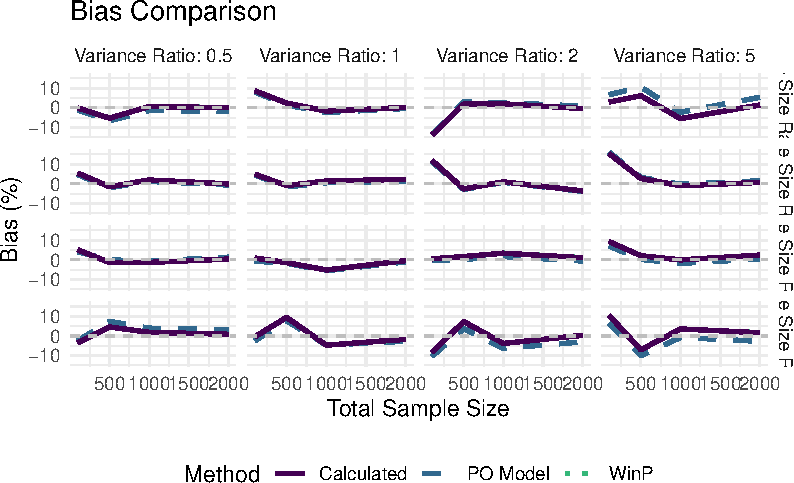
\includegraphics{po-model-sim-Quarto_files/figure-pdf/create-plots-1.pdf}

\begin{Shaded}
\begin{Highlighting}[]
\FunctionTok{print}\NormalTok{(plot\_coverage)}
\end{Highlighting}
\end{Shaded}

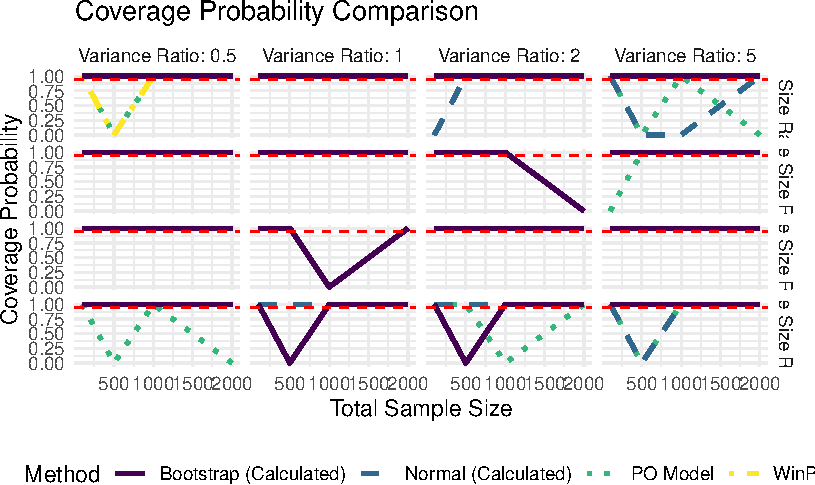
\includegraphics{po-model-sim-Quarto_files/figure-pdf/create-plots-2.pdf}

\begin{Shaded}
\begin{Highlighting}[]
\CommentTok{\# Save the plots}
\FunctionTok{ggsave}\NormalTok{(}\StringTok{"c\_index\_bias\_comparison\_plot.jpg"}\NormalTok{, plot\_bias, }\AttributeTok{width =} \DecValTok{12}\NormalTok{, }\AttributeTok{height =} \DecValTok{10}\NormalTok{, }\AttributeTok{dpi =} \DecValTok{300}\NormalTok{)}
\FunctionTok{ggsave}\NormalTok{(}\StringTok{"c\_index\_coverage\_comparison\_plot.jpg"}\NormalTok{, plot\_coverage, }\AttributeTok{width =} \DecValTok{12}\NormalTok{, }\AttributeTok{height =} \DecValTok{10}\NormalTok{, }\AttributeTok{dpi =} \DecValTok{300}\NormalTok{)}
\end{Highlighting}
\end{Shaded}

\subsection{Final Summary Statistics}\label{final-summary-statistics}

\begin{Shaded}
\begin{Highlighting}[]
\CommentTok{\# Print final summary statistics}
\NormalTok{summary\_stats }\OtherTok{\textless{}{-}}\NormalTok{ all\_results }\SpecialCharTok{\%\textgreater{}\%}
  \FunctionTok{group\_by}\NormalTok{(TotalSampleSize, Ratio, VarRatio) }\SpecialCharTok{\%\textgreater{}\%}
  \FunctionTok{summarise}\NormalTok{(}\FunctionTok{across}\NormalTok{(}\FunctionTok{c}\NormalTok{(TrueConc, }
\NormalTok{                     BiasApprox, }
\NormalTok{                     BiasWinP, }
\NormalTok{                     BiasConc,}
\NormalTok{                     CoverageApprox, }
\NormalTok{                     CoverageWinP, }
\NormalTok{                     CoverageConcNormal, }
\NormalTok{                     CoverageConcBoot), }
\NormalTok{                   mean, }\AttributeTok{.names =} \StringTok{"mean\_\{.col\}"}\NormalTok{),}
            \AttributeTok{ValidRuns =} \FunctionTok{first}\NormalTok{(ValidRuns),}
            \AttributeTok{.groups =} \StringTok{\textquotesingle{}drop\textquotesingle{}}\NormalTok{) }\SpecialCharTok{\%\textgreater{}\%}
  \FunctionTok{rename}\NormalTok{(}
    \StringTok{\textasciigrave{}}\AttributeTok{Bias PO Model}\StringTok{\textasciigrave{}} \OtherTok{=}\NormalTok{ mean\_BiasApprox,}
\StringTok{\textasciigrave{}}\AttributeTok{Bias WinP}\StringTok{\textasciigrave{}} \OtherTok{=}\NormalTok{ mean\_BiasWinP,}
    \StringTok{\textasciigrave{}}\AttributeTok{Bias Normal}\StringTok{\textasciigrave{}} \OtherTok{=}\NormalTok{ mean\_BiasConc,}
    \StringTok{\textasciigrave{}}\AttributeTok{Coverage PO Model}\StringTok{\textasciigrave{}} \OtherTok{=}\NormalTok{ mean\_CoverageApprox,}
    \StringTok{\textasciigrave{}}\AttributeTok{Coverage WinP}\StringTok{\textasciigrave{}} \OtherTok{=}\NormalTok{ mean\_CoverageWinP,}
    \StringTok{\textasciigrave{}}\AttributeTok{Coverage Normal}\StringTok{\textasciigrave{}} \OtherTok{=}\NormalTok{ mean\_CoverageConcNormal,}
    \StringTok{\textasciigrave{}}\AttributeTok{Coverage Bootstrap}\StringTok{\textasciigrave{}} \OtherTok{=}\NormalTok{ mean\_CoverageConcBoot}
\NormalTok{  ) }\SpecialCharTok{\%\textgreater{}\%}
  \FunctionTok{arrange}\NormalTok{(TotalSampleSize, Ratio, VarRatio)}

\FunctionTok{print}\NormalTok{(summary\_stats)}
\end{Highlighting}
\end{Shaded}

\begin{verbatim}
# A tibble: 64 x 12
   TotalSampleSize Ratio VarRatio mean_TrueConc `Bias PO Model` `Bias WinP`
             <dbl> <fct> <fct>            <dbl>           <dbl>       <dbl>
 1             100 0.5   0.5              0.793          -1.10       -0.119
 2             100 0.5   1                0.760           8.04        8.63 
 3             100 0.5   2                0.718         -13.8       -13.9  
 4             100 0.5   5                0.658           6.65        2.90 
 5             100 1     0.5              0.793           4.63        5.44 
 6             100 1     1                0.760           4.48        4.86 
 7             100 1     2                0.718          11.3        11.9  
 8             100 1     5                0.658          16.0        15.4  
 9             100 2     0.5              0.793           4.14        5.13 
10             100 2     1                0.760          -0.624       0.898
# i 54 more rows
# i 6 more variables: `Bias Normal` <dbl>, `Coverage PO Model` <dbl>,
#   `Coverage WinP` <dbl>, `Coverage Normal` <dbl>, `Coverage Bootstrap` <dbl>,
#   ValidRuns <dbl>
\end{verbatim}

\begin{Shaded}
\begin{Highlighting}[]
\CommentTok{\# Save the summary statistics}
\FunctionTok{write.csv}\NormalTok{(summary\_stats, }\StringTok{"final\_summary\_statistics.csv"}\NormalTok{, }\AttributeTok{row.names =} \ConstantTok{FALSE}\NormalTok{)}
\end{Highlighting}
\end{Shaded}




\end{document}
